\documentclass[onepage, 12pt]{beamer}
\mode<presentation>{
	\setbeamercovered{transparent}
	%\beamertemplatenavigationsymbolsempty
	\setbeamertemplate{footline}[frame number]
% 	\usefonttheme{professionalfonts}
}


% % https://tex.stackexchange.com/questions/446063/change-background-colour-to-black-and-text-to-white
% \usecolortheme{owl}

% https://tex.stackexchange.com/questions/34166/understanding-minipages-aligning-at-top
\usepackage{adjustbox}

% https://tex.stackexchange.com/questions/124256/how-do-i-get-numbered-entries-in-a-beamer-bibliography
\setbeamertemplate{bibliography item}{\insertbiblabel}

% https://tex.stackexchange.com/questions/49048/how-to-cite-one-bibentry-in-full-length-in-the-body-text
\usepackage{bibentry}
\bibliographystyle{plain}
\nobibliography*
%
% https://tex.stackexchange.com/questions/163827/wrong-vertical-spaces-using-bibentry-within-beamer/163842
\def\mybeamernewblock{%
  \usebeamercolor[fg]{bibliography entry author}%
  \usebeamerfont{bibliography entry author}%
  \usebeamertemplate{bibliography entry author}%
  \def\newblock{%
    \usebeamercolor[fg]{bibliography entry title}%
    \usebeamerfont{bibliography entry title}%
    \usebeamertemplate{bibliography entry title}%
    \def\newblock{%
      \usebeamercolor[fg]{bibliography entry location}%
      \usebeamerfont{bibliography entry location}%
      \usebeamertemplate{bibliography entry location}%
      \def\newblock{%
        \usebeamercolor[fg]{bibliography entry note}%
        \usebeamerfont{bibliography entry note}%
        \usebeamertemplate{bibliography entry note}}}}%
  \leavevmode
}
\newenvironment{references}{\begin{itemize}\let\newblock\mybeamernewblock}{\end{itemize}}


\setbeamersize{text margin left=10pt, text margin right=10pt}
\setbeamertemplate{itemize items}[circle]

\beamertemplatenavigationsymbolsempty

% http://tex.stackexchange.com/questions/8680/how-can-i-insert-a-newline-in-a-framebox
%\usepackage{minibox}
%\usepackage{framed}
%\usepackage[usestackEOL]{stackengine}

% https://tex.stackexchange.com/questions/433450/how-to-frame-any-environment-like-minipage-and-others
\usepackage{framed}

% % https://tex.stackexchange.com/questions/91124/itemize-removing-natural-indent
% \usepackage{enumitem}

% % http://tex.stackexchange.com/questions/167000/annotating-tables-with-tikz-adding-arrows
% \usepackage{color, colortbl}
\usepackage{tikz}
\tikzstyle{every picture}+=[remember picture]
%\usetikzlibrary{tikzmark, positioning, fit, shapes.misc}

%% http://tex.stackexchange.com/questions/91124/itemize-removing-natural-indent
%\usepackage{enumitem}

%% http://tex.stackexchange.com/questions/41408/a-five-level-deep-list
%\usepackage{enumitem}
%\setlistdepth{9}

% https://tex.stackexchange.com/questions/20792/how-to-superimpose-latex-on-a-picture
\usepackage{overpic}

% % http://tex.stackexchange.com/questions/32661/how-to-locate-figures-with-x-y-specified-location-in-a-presentation
% \usepackage[absolute,overlay]{textpos} % absolute positioning of stuff
% \setlength{\TPHorizModule}{1mm}
% \setlength{\TPVertModule}{1mm}

\usepackage{graphicx}
\graphicspath{{../img/}}
\AtBeginDocument{\DeclareGraphicsExtensions{.eps, .png, .gif, .pdf, .jpg}}

\usepackage[makeroom]{cancel}

\usepackage[english]{babel}
\usepackage[T1]{fontenc}
\usepackage{times}

% \usepackage{amssymb}
% \usepackage{nicefrac}
% \usepackage{bbm}
% \usepackage{esint}
% \usepackage{sidecap}

\usepackage{hyperref}
% \hypersetup{pdfpagemode=FullScreen}

\newcommand{\HIDE}[1]{}

\newcommand{\skipline}{{\ }\\}

\author{RA}
\subject{Talks}

\newcommand{\CITE}[1]{{\footnotesize[#1]}}

% \input{definitions}

\providecommand{\DIV}{\mathop{\text{div}}}
\providecommand{\GRAD}{\mathop{\text{grad}}}

\providecommand{\IE}{\mathbb{E}}
\providecommand{\IP}{\mathbb{P}}
\providecommand{\IR}{\mathbb{R}}
\providecommand{\IZ}{\mathbb{Z}}

\providecommand{\duality}[2]{\langle #1 \rangle_{#2}}
\providecommand{\norm}[2]{\| #1 \|_{#2}}
\providecommand{\seminorm}[2]{| #1 |_{#2}}
\providecommand{\VERT}{\ensuremath{| \! | \! |}}
\newcommand{\tnorm}[2]{\VERT{#1}\VERT_{{#2}}}

\newcommand{\cA}{\mathcal{A}}
\newcommand{\cB}{\mathcal{B}}
\newcommand{\cL}{\mathcal{L}}
\newcommand{\cN}{\mathcal{N}}
\newcommand{\cT}{\mathcal{T}}
\newcommand{\cX}{\mathcal{X}}
\newcommand{\cY}{\mathcal{Y}}

\providecommand{\Abf}{\mathbf{A}}
\providecommand{\Bbf}{\mathbf{B}}
\providecommand{\Dbf}{\mathbf{D}}
\providecommand{\Ibf}{\mathbf{I}}
\providecommand{\Jbf}{\mathbf{J}}
\providecommand{\Fbf}{\mathbf{F}}
\providecommand{\Hbf}{\mathbf{H}}
\providecommand{\Mbf}{\mathbf{M}}
\providecommand{\Tbf}{\mathbf{T}}
\providecommand{\Pbf}{\mathbf{P}}
\providecommand{\Vbf}{\mathbf{V}}
\providecommand{\pbf}{\mathbf{p}}
\providecommand{\ubf}{\mathbf{u}}
\providecommand{\vbf}{\mathbf{v}}
\providecommand{\wbf}{\mathbf{w}}
\providecommand{\ybf}{\mathbf{y}}
\providecommand{\zbf}{\mathbf{z}}

\renewcommand{\vec}[1]{\mathbf{#1}}

\newcommand{\from}{\colon}

\providecommand{\T}{\mathsf{T}}

\renewcommand{\hat}[1]{\widehat{#1}}
\renewcommand{\tilde}[1]{\widetilde{#1}}

\newcommand{\rd}{\,\mathrm{d}}

\newcommand{\TEXT}[1]{\quad\text{#1}\quad}

% http://tex.stackexchange.com/questions/211518/beamer-vfill-and-itemize
\def\Bottom#1{\vskip 0pt plus 1filll #1}
\def\BottomRight#1{\Bottom{\hfill #1}}

% CODE LISTING
\usepackage{color}
\definecolor{DarkBlue}{rgb}{0,0,0.4}
\definecolor{DarkRed}{rgb}{0.3,0,0}
\definecolor{DarkGreen}{rgb}{0,0.3,0}
\usepackage{listings}
\lstset{%
	language=Python,
	basicstyle=\bf\ttfamily\footnotesize,
	keywordstyle=\color{DarkBlue},
	numbers=left, numberstyle=\footnotesize, numbersep=4pt,
	commentstyle={\color{DarkGreen}},
% 	backgroundcolor=\color{white},
	showspaces=false, showstringspaces=false, showtabs=false,
	frame=none,
	tabsize=4,
	breaklines=true, breakatwhitespace=false,
	emphstyle={[1]\color{blue}},
	emphstyle={[2]\color{DarkGreen}},
	%morekeywords={parfor,true,false},
	xleftmargin=8pt,
	numbers=none
}


%%%%%%%%%%%%%%%%%%%%%%%%%%%%%%%%%%%%%%%%%%%%%%%%%%%%%%%%%%%%%%%%%%%%%%%%%%%%%%%%
%%
%%%%%%%%%%%%%%%%%%%%%%%%%%%%%%%%%%%%%%%%%%%%%%%%%%%%%%%%%%%%%%%%%%%%%%%%%%%%%%%%

\usepackage{ifthen}

\newcommand{\REDBOX}[1]{
	\setlength{\fboxrule}{1pt}
	\fcolorbox{red}{SeeMeBarely}{$\displaystyle
		#1
	$}
}

\definecolor{SeeMeBarely}{RGB}{230,230,230}
\definecolor{Purple}{RGB}{128,0,128}
\definecolor{DeepPurple}{RGB}{32,0,96}
\newcommand{\ra}[1]{{\color{blue}{#1}}}
\newcommand{\cred}[1]{{\color{red}{#1}}}
\newcommand{\cblu}[1]{{\color{blue}{#1}}}
\newcommand{\cpur}[1]{{\color{Purple}{#1}}}

\DeclareMathOperator*{\argmin}{arg\,min}

\newcommand{\ItemComment}[1]{\hfill{\scriptsize(#1)\normalsize}}


% http://www.webnots.com/vibgyor-rainbow-color-codes/
\definecolor{a}{RGB}{148, 0, 211}
\definecolor{b}{RGB}{75, 0, 130}
\definecolor{c}{RGB}{0, 0, 255}
\definecolor{d}{RGB}{0, 160, 0}
\definecolor{e}{RGB}{200, 200, 0}
\definecolor{f}{RGB}{255, 127, 0}
\definecolor{g}{RGB}{255, 0, 0}
%
\definecolor{z}{RGB}{0, 0, 0}
\definecolor{w}{RGB}{255, 255, 255}

% % http://tex.stackexchange.com/questions/17611/how-does-one-type-chinese-in-latex
% \usepackage{CJKutf8}
% \AtBeginDvi{\input{zhwinfonts}}
% %
% \newcommand{\REN}{\begin{CJK*}{UTF8}{gbsn}人\end{CJK*}}
% \newcommand{\ren}[1]{{\color{#1}\REN}}



%%%%%%%%%%%%%%%%%%%%%%%%%%%%%%%%%%%%%%%%%%%%%%%%%%%%%%%%%%%%%%%%%%%%%%%%%%%%%%%%
\begin{document}
%%%%%%%%%%%%%%%%%%%%%%%%%%%%%%%%%%%%%%%%%%%%%%%%%%%%%%%%%%%%%%%%%%%%%%%%%%%%%%%%
%%%%%%%%%%%%%%%%%%%%%%%%%%%%%%%%%%%%%%%%%%%%%%%%%%%%%%%%%%%%%%%%%%%%%%%%%%%%%%%%


\begin{frame}[plain,t]
	\begin{center}
        \vspace{1cm}
		%\small
		%
		Abject mismatch tester gets us
		\\
		{\small\color{gray} Masterclass -- session V}
		%
% 		\\[1\baselineskip]
% 		\small
% 		RA
% 		\\[1\baselineskip]
% 		\footnotesize
% 		\EMAIL

		\vspace{1cm}
		%

	\end{center}
	
	
	\Bottom{
		\scriptsize
		R.A.
		\hfill
		BSM, Mar 12, 2020
		\\ {\ }
	}
\end{frame}


%%%%%%%%%%%%%%%%%%%%%%%%%%%%%%%%%%%%%%%%%%%%%%%%%%%%%%%%%%%%%%%%%%%%%%%%%%%%


% \begin{frame}{}{}
%     Find and solve a differential equation
%     for the curve in the $x$-$t$ plane
%     that goes
%     through $(c, 0)$
%     and is perpendicular
%     to the solution curves of $\dot{x}(t) = -x(t)$.
% \end{frame}



\begin{frame}[t]{}{}
	 A large class is to be divided into teams and each student must be a member of exactly one team. However, each student dislikes three of their classmates. 
	 How many teams must be created so that no student is the teammate of someone they dislike?
	 
	 Dislike need not be mutual. Teams need not be equally sized.

	\Bottom{%
		[2019-Rambo, \#14]
	}
\end{frame}


\begin{frame}[t]{}{}
	What is the radius of convergence of
	\begin{align*}
		\sum_{n \geq 0}
		\frac{
			(n x)^n
		}{
			2 \times 4 \times 6 \times \dots \times 2n
		}
	\end{align*}

    
	\Bottom{%
		[2019-Rambo, \#40]
	}
\end{frame}


\begin{frame}[t]{}{}
	Let $X_i$ be binary iid rv with $p = \tfrac12$,
	and set $X = X_1 + \ldots + X_{100}$.
	
	Which is largest?
	
	\begin{itemize}
	\item $\text{Var}(X)$
	\item $100 \times \mathbb{P}(|X - 50| > 25)$
	\item $100 \times \mathbb{P}(X \geq 60)$
	\item $\sum_{k \geq 0} \frac{k}{2^k} {100 \choose k}$
	\item $30$
	\end{itemize}

	\Bottom{%
		[2019-Rambo, \#56]
	}
\end{frame}


\begin{frame}[t]{}{}
	Compute
	\begin{align*}
		\lim_{n \to \infty}
		\frac{1}{n}
		+
		\frac{1}{2 + n}
		+
		\frac{1}{4 + n}
		+
		\ldots
		+
		\frac{1}{3 n}
	\end{align*}
    
	\Bottom{%
		[2019-Rambo, \#57]
	}
\end{frame}


\begin{frame}[t]{}{}
	\begin{center}
		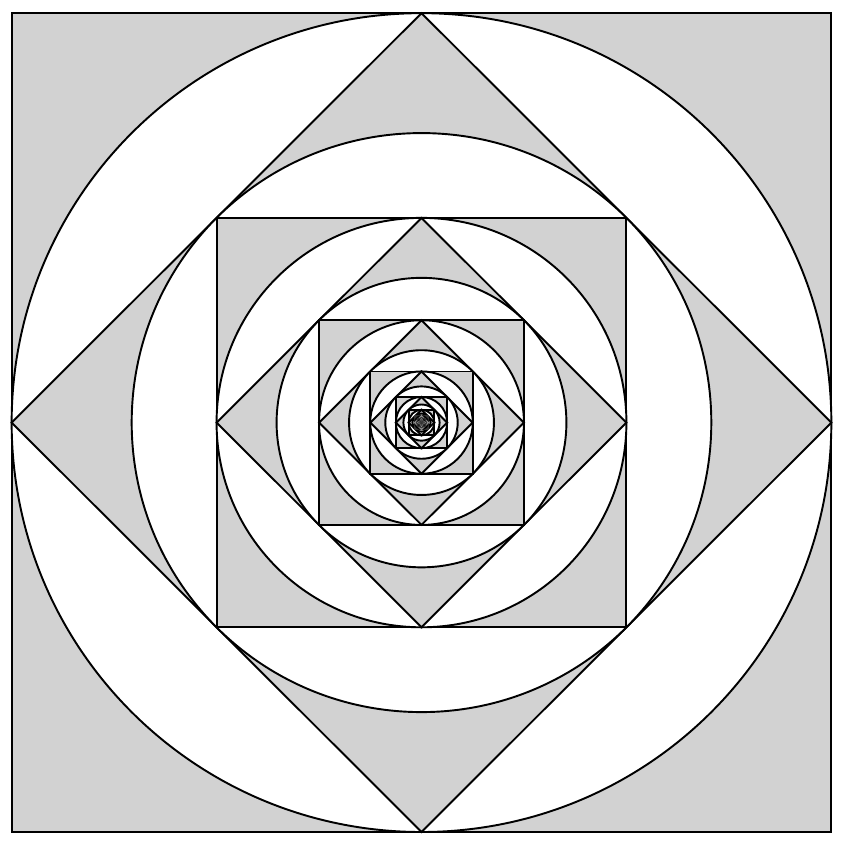
\includegraphics[width=0.5\textwidth]{pattern}
	\end{center}
    
	\Bottom{%
		[2019-Rambo, \#65]
	}
\end{frame}


\begin{frame}{}{}
    Give the maximal interval of existence $(0, t^\star)$
    for the initial value problem
    $\dot{x}(t) = x^2(t)$
    with
    $x(0) := x_0 > 0$.
    %
    Can you continue the solution past the blow up time?

    {\ }
    
    \pause
    
    Now consider 
    $\dot{z}(t) = z^2(t)$, $t > 0$,
    for a complex-valued function $z$
    with the intial value
    $z(0) = x_0 + i \epsilon$,
    where $x_0 > 0$ and $\epsilon \neq 0$ are real.
    %
    Where needed, assume $x_0 = 1$.

    \begin{itemize}
    \item 
        What happens to the blow up time?
    \item
        Decomposing $z = x + i y$,
        write down the differential equations for $x$ and $y$.
%     \item
%         Argue that $x^2(t) + (y(t) - R_0)^2 = R_0^2$
%         for a certain real constant $R_0$.
    \item
        Find the trajectory $\{ (x(t), y(t)) : t > 0 \} \subset \mathbb{R}^2$.
    \item
        Sketch the evolution in $(t, x, y)$-space 
        for a small $\epsilon > 0$.
        %
        What happens for $\epsilon \searrow 0$?
    \end{itemize}
\end{frame}



\begin{frame}{}{}
    \begin{itemize}
    \item 
        $\cos(y) - \frac{dy}{dx}x \sin(y) + \frac{dy}{dx}y^2 = 0$
    \item
        $\frac{dy}{dx} = \frac{x^2-x+y^2}{e^y-2xy}$
    \item
        $\frac{dy}{dx} + e^{3x} - 4y = 0$
    \item
        $x \frac{dy}{dx} + (x+1)y = 3 \quad (x<0)$
    \item
        $\frac{dy}{dx} = 1 - \frac{y}{x}$
    \item
        $\frac{dy}{dx} = \frac{y-x}{y+x} \quad (x>0)$
    \item
        $y''-y' -12y = 0$
    \item
        $y'' - 4y' + 9y = 0$
    \item
        $y''-6y'+9y = 0$
    \item
        $y''-5y' +6y = 3x + 3$
    \item 
        $y''-5y' +6y = e^{4x}$
    \item
        stability of equilibria of $\frac{dP}{dt} = P(P-5)(P-7)$
    \end{itemize}
    
    \hfill
    {\footnotesize [C.~Tompkins]}
\end{frame}



%%%%%%%%%%%%%%%%%%%%%%%%%%%%%%%%%%%%%%%%%%%%%%%%%%%%%%%%%%%%%%%%%%%%%%%%%%%%%%%%%
%\section{Extra}
%%%%%%%%%%%%%%%%%%%%%%%%%%%%%%%%%%%%%%%%%%%%%%%%%%%%%%%%%%%%%%%%%%%%%%%%%%%%%%%%%
%
%
\newcounter{finalframe}
\setcounter{finalframe}{\value{framenumber}}
% Backup frames follow
%
%
% \begin{frame}
% 	Appendix
% \end{frame}
%
%%
%
%\begin{frame}
%	%
%\end{frame}
%
%
% FINAL SLIDE
\setbeamercolor{background canvas}{bg=black}
\begin{frame}[plain,b]
	\hfill
	\tiny
	\color{gray}
	this slide is intentionally left blank
\end{frame}
\setbeamercolor{background canvas}{bg=white}


%%%%%%%%%%%%%%%%%%%%%%%%%%%%%%%%%%%%%%%%%%%%%%%%%%%%%%%%%%%%%%%%%%%%%%%%%%%%%%%%%
%\section{Bibliography}
%%%%%%%%%%%%%%%%%%%%%%%%%%%%%%%%%%%%%%%%%%%%%%%%%%%%%%%%%%%%%%%%%%%%%%%%%%%%%%%%%

% {
% \tiny
% \bibliography{../../../r/refs}
% }


%%%%%%%%%%%%%%%%%%%%%%%%%%%%%%%%%%%%%%%%%%%%%%%%%%%%%%%%%%%%%%%%%%%%%%%%%%%%%%%%
\setcounter{framenumber}{\value{finalframe}}
\end{document}
%%%%%%%%%%%%%%%%%%%%%%%%%%%%%%%%%%%%%%%%%%%%%%%%%%%%%%%%%%%%%%%%%%%%%%%%%%%%%%%%
%%%%%%%%%%%%%%%%%%%%%%%%%%%%%%%%%%%%%%%%%%%%%%%%%%%%%%%%%%%%%%%%%%%%%%%%%%%%%%%%

